\begin{figure}[h!]
\begin{center}
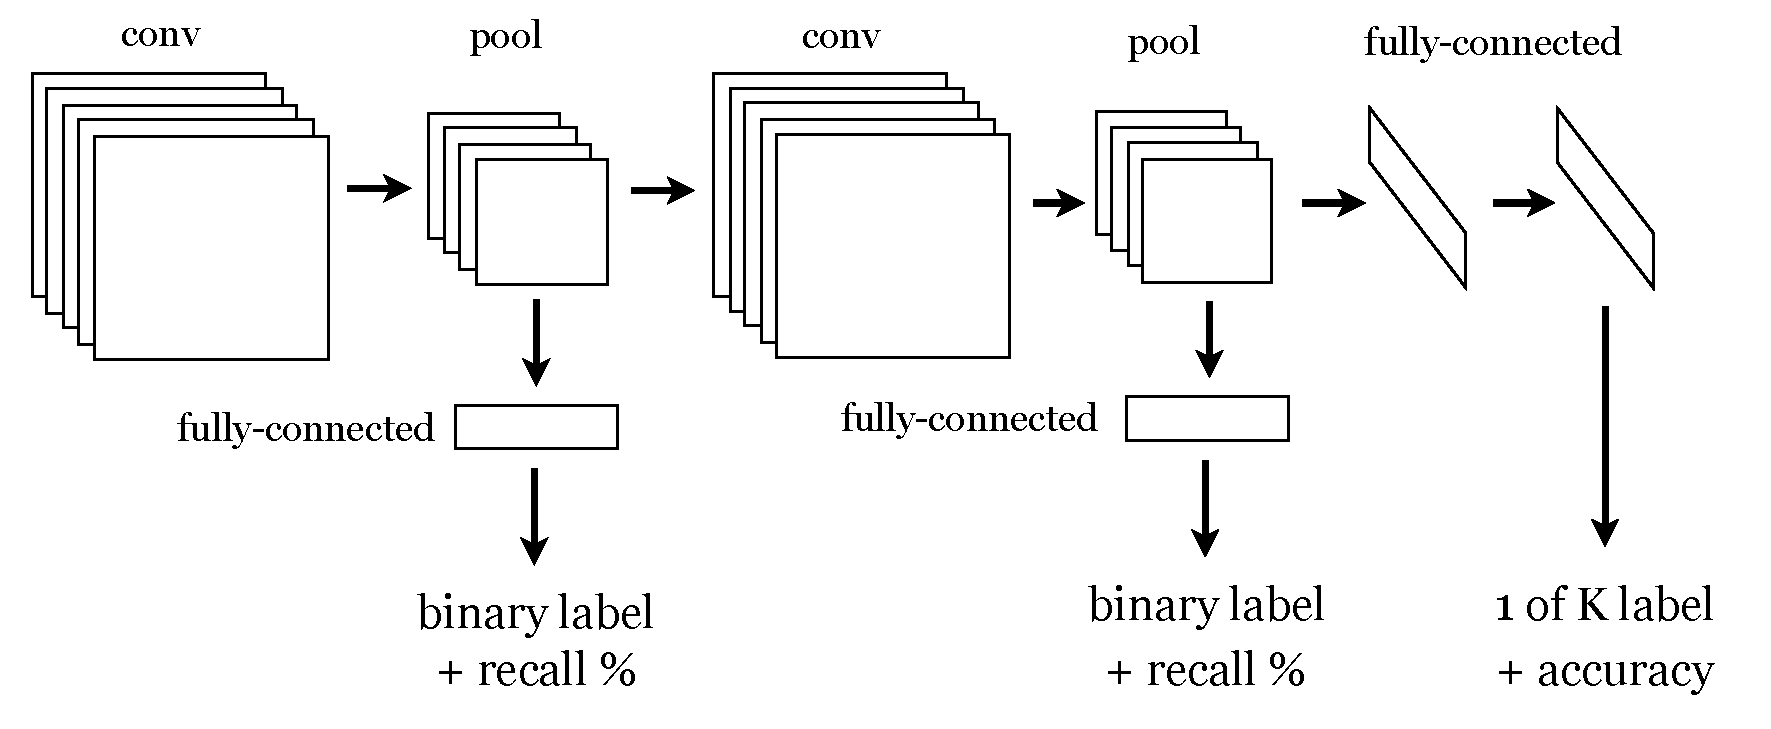
\includegraphics[width=0.98\columnwidth]{../ccnn/figures/ccnn-expanded.pdf}
\caption{
The Cascade CNN has a Reject option after computationally expensive layers, implemented as a binary prediction for reject/keep (background/foreground for our detection task).
The goal of the Reject layer is to maintain high recall while culling as much of the batch as possible, so that we can avoid doing as much convolution in the next layer.
}\label{fig:ccnn}
\end{center}
\end{figure}
